\documentclass[ngerman,inputenc]{beamer}

\usepackage{amsmath, amssymb}
\usepackage{appendix}
\usepackage{pstricks}
\usepackage[utf8]{inputenc}
\usepackage{tikz}

\usepackage{graphicx} %package to manage images
\graphicspath{{images/}}

\definecolor{darkblue}{cmyk}{1.0,0.3,0,0.5}
\definecolor{darkred}{cmyk}{0.25,1,0.1,0.1}
\definecolor{uniblau}{cmyk}{1.0,0.7,0.1,0.6}
\definecolor{unihellblau}{cmyk}{0.2,0.14,0,0}
\definecolor{unihellhellblau}{cmyk}{0.05,0.035,0,0}
\definecolor{darkerblue}{cmyk}{1.0,0.3,0,0.7}

\setbeamertemplate{headline}{
\setbeamercolor{author in head/foot}{fg=white,bg=uniblau!80}
 \hbox{%
  \begin{beamercolorbox}[wd=\paperwidth,ht=2.25ex,dp=1ex,left]{author in head/foot}%
    \usebeamerfont{author in head/foot} \hspace{3pt} \insertsection%
  \end{beamercolorbox}
  }
}

\setbeamertemplate{frametitle}
{
    \setbeamercolor{frametitle}{fg=white,bg=uniblau}
    \vspace{-0.1em}
  \begin{beamercolorbox}[wd=\paperwidth,ht=3ex,dp=2ex,left]{frametitle}%
    \usebeamerfont{frametitle}\hspace{0.7em} \textbf{\insertframetitle}%
  \end{beamercolorbox}%
}

\setbeamertemplate{footline}
{
  \leavevmode%
   \hspace{-1em}
  \hbox{%
    \setbeamercolor{author in head/foot}{fg=white,bg=uniblau!60}
  \begin{beamercolorbox}[wd=.42\paperwidth,ht=2.25ex,dp=1	ex,center]{author in head/foot}%
    \usebeamerfont{author in head/foot}\insertshortauthor~~(\insertshortinstitute)
  \end{beamercolorbox}%
  \hspace{-1em}
\setbeamercolor{title in head/foot}{fg=white,bg=uniblau!80}
  \begin{beamercolorbox}[wd=.35\paperwidth,ht=2.25ex,dp=1ex,center]{title in head/foot}%
    \usebeamerfont{title in head/foot}\insertshorttitle
  \end{beamercolorbox}%
  \hspace{-1em}
  \setbeamercolor{date in head/foot}{fg=white,bg=uniblau}
  \begin{beamercolorbox}[wd=.25\paperwidth,ht=2.25ex,dp=1ex,right]{date in head/foot}%
    \usebeamerfont{date in head/foot}\insertshortdate{}\hspace*{1em}
    \insertframenumber{} /
    \inserttotalframenumber\hspace*{2ex}
  \end{beamercolorbox}}%
  \vskip0pt%
}

\let\ueberschrift=\frametitle
\renewcommand\frametitle[1]{%
  \ueberschrift{
  \rput[l](0,0){#1}
  }
}

\usecolortheme[named=uniblau]{structure}

\title[Airbnb Oslo]{Price Predictions on Airbnb Accomodations in Oslo, Norway}
\date{21.02.2022}
\author[Freitag, Beck]{Marei Freitag, Joel Beck}
\institute[University Göttingen]{Georg-August-University of Göttingen}

% display TOC before every section and subsection without duplicates
% https://stackoverflow.com/questions/2795478/latex-beamer-prevent-showing-the-toc-at-one-occasion

\RequirePackage{ifthen}
\newboolean{sectiontoc}
\setboolean{sectiontoc}{true} % default to true

\AtBeginSection[]
{
  \ifthenelse{\boolean{sectiontoc}}{
  \begin{frame}
    \frametitle{Table of Contents}
    \tableofcontents[currentsection, currentsubsection, subsubsectionstyle={show/show/shaded/shaded}]
  \end{frame}
  }
}

\AtBeginSubsection[]
{
  \begin{frame}
    \frametitle{Table of Contents}
    \tableofcontents[currentsection, currentsubsection, subsubsectionstyle={show/show/shaded/shaded}]
  \end{frame}
}

\newcommand{\toclesssection}[1]{
  \setboolean{sectiontoc}{false}
  \section{#1}
  \setboolean{sectiontoc}{true}
}


\begin{document}

\begin{frame}
  \titlepage
\end{frame}


\begin{frame}
  \frametitle{Table of Contents}
  \tableofcontents
\end{frame}

%%%%%%%%%%%%%%%%%%%%%%%%% Kapteil 1 %%%%%%%%%%%%%%%%%%%%%%%%%

\toclesssection{1. Introduction}

\begin{frame}{Introduction}

  Aims of this work:
  \begin{itemize}
    \item Establish a deep learning approach to predict the price of an accomodation per night
    \item Focus on explainability and interpretability
  \end{itemize}
  \hspace{12pt}

  $\rightarrow$ Underlying data: provided by Airbnb, contains various information about the listings in Oslo, Norway

\end{frame}


%%%%%%%%%%%%%%%%%%%%%%%%% Kapteil 2: Methods %%%%%%%%%%%%%%%%%%%%%%%%%

\toclesssection{2. Methods}

%%% Data Preprocessing %%%
\subsection{2.1 Preprocessing}

\subsubsection{Feature Engineering}

\begin{frame}{Feature Engineering: Images}

  \begin{itemize}
    \item Use transfer learning on a pretrained CNN (ResNet18) with the first 5 images per listing as input data
    \item Added Fully Connected Network at the end containing three layers and \texttt{ReLU} activation functions to be sure the CNN is able to generalize
    \item Also implemented CNN manually as a benchmark model to compare the results
          % COMMENT: Ergebnisse des selber implementierten CNN?
  \end{itemize}

  \hspace{5pt}

  Results:
  \begin{itemize}
    \item pretrained \texttt{ResNet18} achieved a Mean Absolute Error of $579$ NOK (approx. $58$ Euros) on the Validation Set
          %null model has MAE 630 NOK without log transformation, but 569 NOK with
    \item But correlation of the CNN predictions with the true price is $0.41$
          % at least positive tendencies of the CNN predictions
  \end{itemize}

\end{frame}

\begin{frame}{Image Predictions}

  \begin{figure}[H]
    \centering
    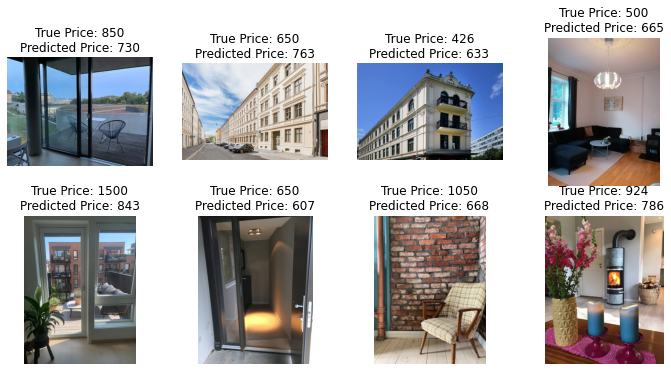
\includegraphics[width=10cm]{cnn_examples_medium.png}
    \caption{CNN example predictions}
  \end{figure}

\end{frame}


\begin{frame}{Feature Engineering: Reviews}
  % Language and Sentiment
  \begin{itemize}
    \item Language: Detect language of each review
    \item Sentiment analysis: Get the sentiment of each review
  \end{itemize}

  \hspace{5pt}

  New features per listing:
  \begin{itemize}
    \item[1.] Number of reviews
    \item[2.] Median review length
    \item[3.] Number of different languages of the reviews as well as a list of the different languages
    \item[4.] Fraction of Norwegian and English reviews
    \item[5.] Ratio of negative reviews to the total number of reviews
  \end{itemize}

\end{frame}

\begin{frame}{Wordclouds of the Reviews}

  % Wordcloud
  \begin{figure}[t]
    \centering
    \begin{minipage}{6.7cm}
      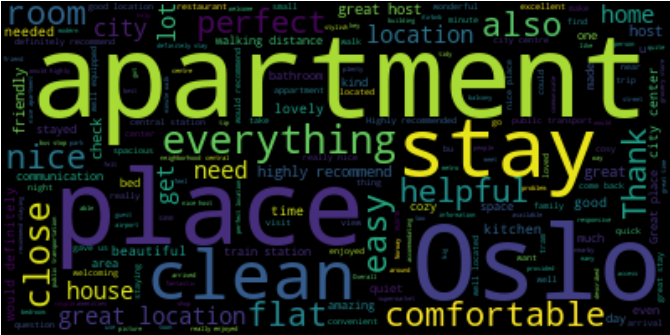
\includegraphics[width=\columnwidth]{wordcloud_eng.png}
    \end{minipage}
    \begin{minipage}{6.7cm}
      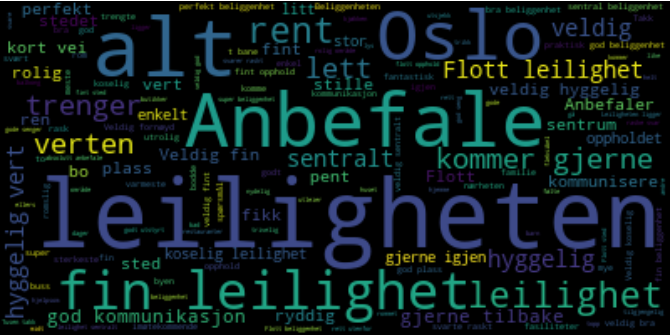
\includegraphics[width=\columnwidth]{wordcloud_nor.png}
    \end{minipage}
    \caption{Wordclouds in English and Norwegian}
    \label{fig:wordclouds}
  \end{figure}

\end{frame}


\subsubsection{Feature Selection}

\begin{frame}{Feature Selection \& Data Cleaning}

  Feature Selection:
  \begin{itemize}
    \item[1.] Manually selected features based on background knowledge, correlation analysis and the number of missing values
      %based on three criteria: background knowledge, there exists correlation between feature and price, not too many missing values because of small dataset
    \item[2.] Adjusted these features by analyzing the results of different feature selection algorithms and fitted auxiliary linear regression % mainly focused on Principal Component Analysis and Recursive Feature Selection
  \end{itemize}

  \hspace{5pt}

  Data Cleaning:
  \begin{itemize}
    \item Converting data types
    \item Splitting text-based variables into more convenient numeric or boolean features
    \item Aggregating rare categories of categorical variables into one larger \emph{Other} group to stabilize estimation % example: property type, just one House Boat with very high price (outlier?)
    \item One-Hot encoding of categorial variables and standardization of numerical variables
  \end{itemize}

\end{frame}


%%% Models %%%

\subsection{2.2 Models}

\subsubsection{Classical Models}

\begin{frame}{Classical Models}
  % In order to get some insights, we selected four classical Machine Learning models of varying complexity from the \texttt{scikit-learn} library \citep{pedregosa2011} to serve as benchmark models for our custom Neural Net.

  \begin{itemize}
    \item[1.] \textbf{Linear Regression}: simple, well understood in terms of underlying theory and highly interpretable.
    \item[2.] \textbf{Ridge Regression}: still very interpretable with a closed form analytical solution; one hyperparameter
    \item[3.] \textbf{Random Forest}: very flexible model with many hyperparameters determining e.g. the number of regression trees and the tree depth, but can be applied to many contexts and often works 'out of the box'
    \item[4.] \textbf{Histogram-Based Gradient Boosting}: modern and fast tree-based gradient boosting algorithm; large number of tunable hyperparameters
      %, some of them similar to the Random Forest parameters, some of them more specific to the \emph{Boosting} instead of the \emph{Bagging} approach such as the learning rate.
      %Similar to the very popular \href{https://xgboost.readthedocs.io/en/stable/}{XGBoost} \citep{chen2016} and \href{https://lightgbm.readthedocs.io/en/latest/}{LightGBM} \citep{ke2017} implementations that regularly outperform deep Neural Networks in Kaggle competitions on tabular data.
  \end{itemize}

\end{frame}


\subsubsection{Neural Network}

\begin{frame}{Neural Network: Model Architecture}

  \begin{columns}
    \begin{column}{0.5\textwidth}
      \begin{itemize}
        %\item Starting from roughly $60$ input features, the network width is first blown up to $256$ features before steadily decreasing it again to a single output neuron in the final layer.
        \item linear input layer (about $60$ features)
        \item $6$ intermediary \textbf{blocks} with $64$, $128$, $256$, $128$, $64$ and $8$ output features:
              \begin{itemize}
                \item[–] residual connection
                \item[–] linear layer with BatchNorm, \texttt{ReLU} activation function and dropout
              \end{itemize}
        \item $1$ output neuron
      \end{itemize}
    \end{column}
    \begin{column}{0.5\textwidth}
      \begin{center}
        \begin{figure}
          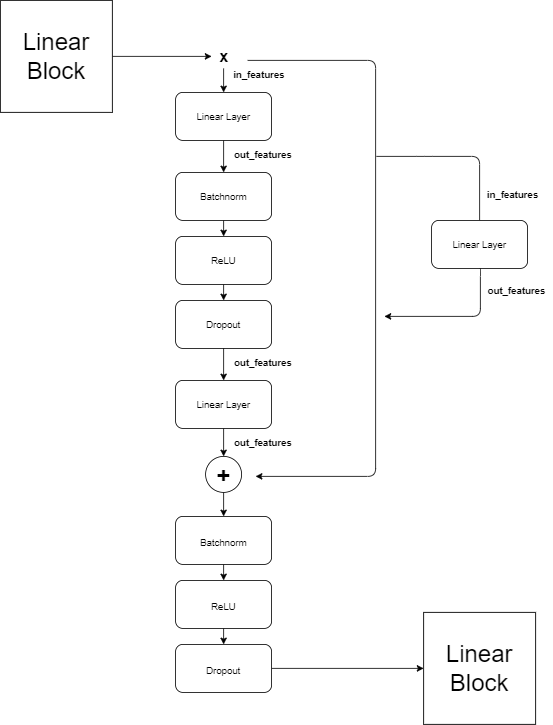
\includegraphics[width=0.9\columnwidth]{mlp_architecture.png}
          \caption{Linear Block in the FC-NN}
        \end{figure}
      \end{center}
    \end{column}
  \end{columns}

\end{frame}

\begin{frame}{Neural Network: Model Training}

  \begin{itemize}
    \item \texttt{Adam} optimizer with learning rate set to 0.01
    \item Loss function: \textit{Mean Squared Error} Loss
    \item Epochs: % COMMENT: wie viele Epochen wurden trainiert?
  \end{itemize}

  % COMMENT: hier auf den Einfluss des Dropouts eingehen?


\end{frame}




%%%%%%%%%%%%%%%%%%%%%%%%% Kapteil 3: Results %%%%%%%%%%%%%%%%%%%%%%%%%

\section{3. Results}

\begin{frame}{Test - Slide 1}

\end{frame}

%%%%%%%%%%%%%%%%%%%%%%%%% Kapteil 4: Conclusion %%%%%%%%%%%%%%%%%%%%%%%%%

\section{4. Conclusion}

\begin{frame}{Test - Slide 2}

\end{frame}


\begin{frame}

  \begin{center}
    \LARGE{\textbf{Thanks for listening!}}\\[10mm]
    \large{Questions?}
  \end{center}

\end{frame}


\end{document}
%
